
%(BEGIN_QUESTION)
% Copyright 2011, Tony R. Kuphaldt, released under the Creative Commons Attribution License (v 1.0)
% This means you may do almost anything with this work of mine, so long as you give me proper credit

Suppose a FOUNDATION Fieldbus pressure transmitter will be used to measure flow through a process line by sensing differential pressure generated by an orifice plate.  The orifice's rated pressure range is 0 to 125 inches water column, while flowing 0 to 230 gallons per minute of liquid.  Due to the differential pressure sensor being mounted at a substantial level below the pipe's centerline, the weight of the liquid inside each of the impulse lines applies an extra 38 inches of water column pressure to both sides of the transmitter (``High'' and ``Low'' equally).  The operator needs to see the flow rate in units of GPM, and does not care to see or know the differential pressure directly sensed by the transmitter:

$$\includegraphics[width=15.5cm]{i01840x01.eps}$$

Complete the configuration table in the above illustration, showing the proper {\tt XD\_Scale}, {\tt OUT\_Scale}, and {\tt L\_Type} parameter values to make the transmitter function as it should in this application.

\underbar{file i01840}
%(END_QUESTION)





%(BEGIN_ANSWER)

{\tt OUT\_Scale} = 0 to 230 GPM

\vskip 10pt

{\tt L\_Type} = Indirect Square Root

\vskip 10pt

{\tt XD\_Scale} = 0 to 125 inches water column

\vskip 10pt

The height difference between the pipe and the transmitter is completely irrelevant, because the extra pressure applied to each port is done so {\it equally} and therefore cancels at the transmitter, since the transmitter is inherently a {\it differential} pressure device.

%(END_ANSWER)





%(BEGIN_NOTES)


%INDEX% Fieldbus, instrument ranging: setting XD_Scale and OUT_Scale parameters for an application

%(END_NOTES)

